\chapter{LPQP for MPE Inference}
\label{sec:lpqp}


In the present chapter we investigate the problem of \acf{MPE} inference in
settings where the \acf{LP} relaxation is not tight. Our approach is based on
augmenting the convex \ac{LP} relaxation by a
non-convex term that penalizes inconsistencies present in the \ac{LP}
formulation. A scalar parameter that can be understood as a temperature,
gradually increases the importance of this penalty term. A similar idea will
also be used in \autoref{sec:maximum_entropy_margin} for learning \acp{CRF}.


%----------------------------------------------------------------------------
\section{Introduction}

We study the problem of \ac{MPE}\index{most probable explanation} or equivalently \acf{MAP} inference in graphical 
models. As introduced in~\autoref{sec:background:inference}, the \ac{MPE}
task is to compute a minimum energy\index{energy!minimization} assignment of a set of dependent variables.
In the general case, \ac{MPE} inference
is intractable, and therefore most of the current research efforts are concentrated 
on finding efficient and accurate approximation algorithms. In recent years, 
\acf{LP} relaxations (see \autoref{sec:background:variational_outer}) gained
popularity due to their proven success
in relevant applications. Several efficient algorithms have been developed  
to solve the linear program emerging from the relaxation. 
Despite their success, in many practical problems the solution attained by the
\ac{LP} relaxations is still far from the global minimum.

Our work improves over the \ac{LP} relaxation by leveraging on a second class of
relaxations, namely the \acf{QP} relaxation (see
\autoref{sec:background:variational_inner}). The \ac{QP} 
formulation offers a concise and compact description of the \ac{MPE} problem. 
We formulate a joint \ac{LP} and \ac{QP} \ac{MPE} objective, that encourages auxiliary variables
present in the \ac{LP} relaxation, to agree with their counterpart in the
\ac{QP} relaxation, 
through a penalty function. Despite of the non-convexity of this objective, we 
show that by slowly increasing the weight of the penalty, 
the solutions found are either competitive with, or in most cases better than 
the \ac{LP} relaxation solutions. This is in general not the case for the few existing 
\ac{QP} relaxation solvers. 

We propose two variants of the penalty function, each leading to a
different \ac{LPQP} objective. We show that the resulting non-convex objectives can be 
decomposed into a difference of convex functions, which we solve using the
\acf{CCCP}. Having mastered the non-convexity with the
\ac{CCCP}, we solve one of the remaining convex problems with the dual decomposition method,
and show that the other can be addressed with the norm-product belief propagation.
Interestingly, the main computational task of both of 
the resulting \ac{LPQP} algorithms, turns out to be solving known entropy-augmented
\acp{LP}. 

Our contributions are as follows: First we introduce a combined
\ac{LPQP} objective, incorporating the \ac{QP} constraints through a soft penalty
function in the objective. We propose two alternatives for the penalty function, which
differ in the way the edges in the graph are weighted. Secondly, we derive
\ac{CCCP} based algorithms for the \ac{LPQP} objectives, and show that their core
computational effort reduces to current entropy-augmented \ac{LP} solvers. 
This demonstrates that these modern \ac{LP} solvers can in some cases be utilized in a 
smarter way than simply solving the original \ac{LP} relaxation,
leading to possibly faster convergence, as well as lower energy
\ac{MPE} solutions.
Through experiments on various datasets, we demonstrate the performance 
of the suggested \ac{LPQP} \ac{MPE} inference in comparison to other commonly used solvers. 

%----------------------------------------------------------------------------
\section{Background and Notation}

For the sake of clarity we focus on pairwise graphical models. The extension
to higher-order factors is relatively straightforward, at the price of a more
complicated notation and increased complexity due to the larger factors. Also,
we assume that the \emph{energy function is specified explicitly through unary and
pairwise potentials}, rather than implicitly through parameters and feature
functions. Therefore we can state the \ac{MPE} problem as follows:
For an undirected graph $\gmgraph=(\gmvertex,\gmedge)$
assign each node in the graph to a class or category, such that the overall assignment
minimizes an associated energy. 
Let $\outputvar_i$ denote a discrete variable with a finite domain
$\outputdomain_i$, with $|\outputdomain_i|=K$\footnote{For notational convenience we assume
$\outputdomain_i = \{1,\ldots,K\}$; in the experiments we will however also
consider settings where the domain of the variables has different
size.}, representing the assignment of the $i$-th node. 
The \ac{MPE} problem is defined as
\begin{equation}
    \min_{\outputvarv} \sum_{i\in\gmvertex} \potential_i(\outputvar_i) + \sum_{(i,j) \in
    \gmedge} \potential_{ij}(\outputvar_i, \outputvar_j).
    \label{eq:lpqp:integer_qp}
\end{equation}
Where $\potential_i(\outputvar_i)$ and
$\potential_{ij}(\outputvar_i,\outputvar_j)$ are unary
and pairwise potential functions associated with the node and edge
assignments.
Problem~\eqref{eq:lpqp:integer_qp} can be expressed
as an integer quadratic program using a $K$-ary coding:
\begin{align}
    \min_{\marginalvarv} \quad &  \sum_{i\in\gmvertex}
    \potentialv_{i}^{\transpose}\marginalvarv_{i} +
    \sum_{(i,j) \in
    \gmedge} \marginalvarv_{i}^\transpose\potentialm_{ij}
    \marginalvarv_{j}
    \label{eq:lpqp:integer_qp_kary}
    \\
    \text{s.t.} \quad & \marginalvar_{i;k} \in \{0,1\} \quad \forall i,k
    \quad\text{and}\quad \sum_{k}\marginalvar_{i;k} = 1 \quad \forall i. \notag
\end{align}
The pairwise and unary potentials in~\eqref{eq:lpqp:integer_qp_kary}, are represented as a matrix
$\potentialm_{ij}$ and a vector $\potentialv_{i}$, respectively. 

Variational approaches (see~\autoref{sec:background:variational}) to \ac{MPE} inference reformulate the combinatorial
optimization problem in~\eqref{eq:lpqp:integer_qp} as a continuous optimization
problem. The next sections formally define two such approaches, namely 
the \ac{LP} and \ac{QP} relaxations. In general, the \ac{LP} minimization
results in a \emph{lower bound} on the
energy of the global minimizer, while the \ac{QP} results in an \emph{upper
bound}. The constraint set of the two relaxations is illustrated in
~\autoref{fig:lpqp:lp_and_qp_constraint_set}.

\begin{figure}[htb]
    \centering
    \tikzsetnextfilename{lpqp_polytopes}
    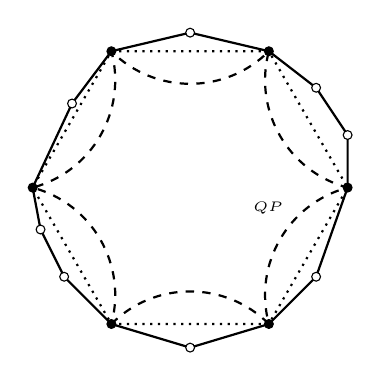
\begin{tikzpicture}[scale=2]
    % outer local marginal polytope
    \draw[thick]
    (0,0) -- (0.5,-0.15) -- (1,0) -- (1.3,0.3) --
    (1.5,0.866) -- (1.5,1.2) -- (1.3,1.5) -- (1,1.732) -- (0.5,1.85) -- (0,1.732) --
    (-0.25,1.4) -- (-0.5,0.866) -- (-0.45,0.6) -- (-0.3,0.3) -- (0,0);

    % marginal polytope
    \draw[thick, dotted]
    (0,0) -- (1,0) --
    (1.5,0.866) -- (1,1.732) -- (0,1.732) -- (-0.5,0.866) -- cycle;

    % inner QP approximation
    \draw[thick,out=45,in=135,relative, dashed]
    (0,0) to (1,0) to
    (1.5,0.866) to (1,1.732) to (0,1.732) to (-0.5,0.866) to (0,0);

    % integer solutions
    \filldraw (0,0) circle (0.8pt);
    \filldraw (1,0) circle (0.8pt);
    \filldraw (1.5,0.866) circle (0.8pt);
    \filldraw (1,1.732) circle (0.8pt);
    \filldraw (0,1.732) circle (0.8pt);
    \filldraw (-0.5,0.866) circle (0.8pt);

    % fractional solutions
    \filldraw[fill=white] (0.5,-0.15) circle (0.8pt);
    \filldraw[fill=white] (1.3,0.3) circle (0.8pt);
    \filldraw[fill=white] (1.5,1.2) circle (0.8pt);
    \filldraw[fill=white] (1.3,1.5) circle (0.8pt);
    \filldraw[fill=white] (0.5,1.85) circle (0.8pt);
    \filldraw[fill=white] (-0.25,1.4) circle (0.8pt);
    \filldraw[fill=white] (-0.45,0.6) circle (0.8pt);
    \filldraw[fill=white] (-0.3,0.3) circle (0.8pt);

    \node (lp) at (1.5,1.5) {\scriptsize$\localmarginalpolytope_{\gmgraph}$};
    \node (ip) at (0.5,0.1) {\scriptsize$\marginalpolytope$};
    \node (qp) at (1,0.7) {\scriptsize$\localmarginalpolytope_{\gmgraph}^{QP}$};
\end{tikzpicture}

    \caption[Constraint set of the LP and QP relaxations]{Schematic
    illustration of the constraint set in the \ac{LP} (solid) and the \ac{QP}
    (dashed) relaxations.
    While the \ac{LP} relaxation is an outer bound on the true marginal
    polytope (dotted) leading to additional fractional solutions (shown as
    non-filled circles), the \ac{QP} relaxation
    gives an inner bound. We use $\localmarginalpolytope_{\gmgraph}^{QP}$ to
    denote the local marginal polytope with additional quadratic consistency
    constraints.}
    \label{fig:lpqp:lp_and_qp_constraint_set}
\end{figure}

\subsection{Linear Programming Relaxation}

The \ac{LP} approach \parencite{Schlesinger1976,Wainwright2008} is
based on a convex relaxation of~\eqref{eq:lpqp:integer_qp_kary}, where an
additional variable $\marginalvarv_{ij}$ is included for each edge.
Proper \emph{local} marginalization is enforced through summation constraints.
Let us define $\potentialv$ as the vectorized version of the matrix
$\potentialm$, i.e.\ $\potentialv = \mathrm{vec}(\potentialm)$
The \ac{LP}\index{linear programming relaxation} reads as
\begin{equation}
    \min_{\marginalvarv\in\localmarginalpolytope_\gmgraph} \sum_{i\in\gmvertex}
    \potentialv_{i}^{\transpose}\marginalvarv_{i} 
    + \sum_{(i,j) \in \gmedge} \potentialv_{ij}^{\transpose}
    \marginalvarv_{ij},
    \label{eq:lpqp:linear_program_relaxation}
\end{equation}
with $\localmarginalpolytope_\gmgraph$, the local marginal polytope:
\[
    \localmarginalpolytope_{\gmgraph} = \left \{ \marginalvarv \left |
    \begin{array}{l}
        \sum_{k} \marginalvar_{i;k} = 1 \quad \forall i \in \gmvertex\\
        \sum_{l} \marginalvar_{ij;kl} = \marginalvar_{i;k} \quad \forall k,
        (i,j)\in\gmedge\\
        \sum_{k} \marginalvar_{ij;kl} = \marginalvar_{j;l} \quad \forall l,
        (i,j)\in\gmedge\\
        \marginalvar_{ij;kl} \geq 0 \quad \forall k,l,(i,j)\in\gmedge\\
    \end{array} \right .
    \right \}.
\]
In the general case, $\localmarginalpolytope_\gmgraph$ is an inexact description of the
marginal polytope $\marginalpolytope$, which requires an exponentially large number of
constraints~\parencite{Wainwright2008}. If $\localmarginalpolytope_\gmgraph$ in
~\eqref{eq:lpqp:linear_program_relaxation} is replaced by
$\marginalpolytope$, then the solution recovers the true \ac{MPE}
assignment. 
A solution to an \ac{LP}-based approach (for a constraint set consisting of any subset of the marginal
polytope, such as $\localmarginalpolytope_\gmgraph$), admits an easy to verify certificate of optimality.
If the solution is integer, it is the global optimum.

The work in~\parencite{Sontag2008} proposes to tighten the polytope by including
summation constraints over larger subsets of variables. This approach has been
successful in identifying the global minimum for some problems.
However, it suffers from an increased complexity as
ultimately an exponentially large set of possible constraints might need to be
searched over. In practice a class of possible summation constraints are
considered, such as those consisting of all triplets.

\subsection{Quadratic Programming Relaxation}
\label{sec:lpqp:qp}

An alternative relaxation of the integer quadratic program
in~\eqref{eq:lpqp:integer_qp_kary} is obtained by simply dropping the integer constraints.
The resulting \ac{QP}\index{quadratic programming relaxation} is given by:
\begin{align}
    \min_{\marginalvarv} \quad &  \sum_{i\in\gmvertex}
    \potentialv_{i}^{\transpose}\marginalvarv_{i} +
    \sum_{(i,j) \in
    \gmedge} \marginalvarv_{i}^\transpose\potentialm_{ij}
    \marginalvarv_{j}
    \label{eq:lpqp:quadratic_program_relaxation}
    \\
    \text{s.t.} \quad & 0 \leq \marginalvar_{i;k} \leq 1 \quad \forall i,k
    \quad\text{and}\quad \sum_{k}\marginalvar_{i;k} = 1 \quad \forall i. \notag
\end{align}
A major advantage of the \ac{QP} relaxation, is its tightness, which means 
that the minimizer 
of~\eqref{eq:lpqp:quadratic_program_relaxation} also minimizes
~\eqref{eq:lpqp:integer_qp},
as was shown in \parencite{Ravikumar2006}. 
The \ac{QP} also benefits from a more compact description compared to the \ac{LP}
relaxation, as it requires fewer constraints and variables to formulate the
\emph{exact} \ac{MPE} problem. The variable vector $\marginalvarv$, is of size 
$K\cdotp|\gmvertex| + K^2\cdotp|\gmedge|$ in the \ac{LP}~\eqref{eq:lpqp:linear_program_relaxation}
and only $K\cdotp|\gmvertex|$ in the \ac{QP}.
The biggest drawback of the \ac{QP} relaxation, 
is that in the general case the optimization problem turns out to be non-convex due to the edges product
term. This fact renders an exact minimization difficult. A \ac{QP} solution is
not necessarily guaranteed to be integer. As was shown
in~\parencite{Ravikumar2006}, a (local) solution to the \ac{QP} relaxation can always
be rounded to an integer solution with smaller or equal energy. We will
discuss this rounding strategy in~\autoref{sec:lpqp:algorithm_overview}.

In terms of motivation, our work is similar to the \ac{QP} 
relaxation approach. The \ac{QP} formulation of the \ac{MPE} problem~\eqref{eq:lpqp:quadratic_program_relaxation}
was introduced in \parencite{Ravikumar2006}, 
but stems from classical mean-field approaches. 
\textcite{Ravikumar2006} solved the non-convex problem
using a convex relaxation. The solution was later improved in \parencite{Kappes2008} 
through a difference of convex functions formulation. Both solvers
are generic in the sense that they do not exploit the graph structure.
Recently \parencite{Kumar2011} introduced a
message-passing algorithm for solving the \ac{QP} relaxation. While improving the 
run time over the other two algorithms, it still generally suffers from poor 
solutions due to local minima.  The \ac{QP} solvers often deal with this drawback 
by restarting with different initializations.
We observed that our \ac{LPQP} algorithms, are much more resilient with respect to 
the initialization. In all of the experiments we conducted, a restart was never required.
We attribute this behavior to the gradual progression between the \ac{LP} and
\ac{QP}.
Finally, in concurrent work~\parencite{Kumar2012} propose a 
hybrid \ac{LP} and \ac{QP} approach to \ac{MPE}, similar to our formulation discussed in the
next section. The resulting optimization problem is solved by a custom
message-passing scheme. Our work on the other hand, in its essence reduces to 
well-known entropy-augmented \ac{LP} objectives, for which efficient
message-passing algorithms exist.


%----------------------------------------------------------------------------
\section{Combined LP and QP Relaxation}

We propose to optimize an objective which is a combination of the \ac{LP} and
\ac{QP}
relaxations. We retain the auxiliary variables $\marginalvarv_{ij}$ of the
pairwise terms, but force these variables to agree with the 
product of the unary marginals $\marginalvarv_i$ and $\marginalvarv_j$. The
constraints, given by $\mathrm{vec}(\marginalvarv_{i} \marginalvarv_{j}^{\transpose}) =
\marginalvarv_{ij} \ \forall (i,j) \in \gmedge$\footnote{Here
$\mathrm{vec}(\marginalvarv_{i}\marginalvarv_{j}^{\transpose})$ denotes the
vectorized version of the outer product of $\marginalvarv_{i}$ and
$\marginalvarv_{j}$.}, are enforced through a penalty function
$\penaltyp(\cdotp)$ incorporated in the objective. The extent to which
the constraint is enforced, is regulated by the parameter $\rho$.

We focus on the \acf{KL} divergence as the penalty function. In
our setting this is equivalent to the mutual information between the unary and
marginal variables. The choice of the penalty function is
motivated by the probabilistic nature of the compared marginal terms.
Moreover, as we will see later, the use of the \ac{KL} divergence as a penalty term
gives rise to efficient message-passing algorithms for the solution of the
resulting optimization problems.
As a reminder, for probability distributions
$\marginalvarv$ and $\bm{\nu}$ of a discrete random variable, 
their \ac{KL} divergence\index{Kullback-Leibler divergence} is defined to be
\[
    \kldivergence(\marginalvarv, \bm{\nu}) \defeq \sum_{k} \marginalvar_{k}
    \log\left(\frac{\marginalvar_{k}}{\nu_{k}}\right).
\]
Our approach enforces consistency between the unary and pairwise marginals for
each edge using the \ac{KL} divergence. As these marginals are properly normalized,
which is ensured
through the constraints in the local marginal polytope, the \ac{KL} divergence
simply corresponds to the
mutual information\index{mutual information} $\mutualinformation$ of the marginals for an edge
$(i,j)$, see~\eqref{eq:background:mutual_information_as_entropy}:
\[
    \mutualinformation_{ij}(\marginalvarv_{ij}, \mathrm{vec}(\marginalvarv_i
    \marginalvarv_j^\transpose)) =
    \entropy(\marginalvarv_i) + \entropy(\marginalvarv_j) -
    \entropy(\marginalvarv_{ij}).
\]
In our work the mutual information between the pairwise term
$\marginalvarv_{ij}$ and the product of unary terms
$\mathrm{vec}(\marginalvarv\marginalvarv^\transpose)$ is
\emph{minimized}, as in the consistent case the mutual information is zero.
The general form of the combined \ac{LPQP} objective reads as 
\begin{equation}
    \min_{\marginalvarv\in\localmarginalpolytope_\gmgraph} 
    \potentialv^{\transpose} \marginalvarv 
    + \rho \penaltyp(\marginalvarv).
    \label{eq:lpqp:combined_objective_scheme}
\end{equation}
The first term is simply the \ac{LP}
objective~\eqref{eq:lpqp:linear_program_relaxation}, written as a scalar product
between the potential function, and the concatenated unary and pairwise
variables. We investigate two constructions of the penalty term
$\penaltyp(\marginalvarv)$. The constructions differ in
the weighting of the edges. The penalty function has the property that it is
positive and only zero if the unary marginals agree with the pairwise
marginals for all the edges.
For $\rho = 0$, \eqref{eq:lpqp:combined_objective_scheme}
amounts to the standard \ac{LP} relaxation. 
On the other extreme when $\rho \to \infty$, the constraints 
$\mathrm{vec}(\marginalvarv_{i} \marginalvarv_{j}^{\transpose}) =
\marginalvarv_{ij} \ \forall (i,j) \in \gmedge$ are fulfilled and the \ac{QP} relaxation is recovered.
By successively increasing $\rho$ during the run of our algorithms, we achieve
a gradual enforcement of the constraints. 

\paragraph{Uniform Weighting} The \ac{KL} divergence is penalized in the same way
for all the edges in the graph:
\begin{align}
    \penaltyp^{\mathit{uni}}(\marginalvarv) & \defeq \sum_{(i,j) \in \gmedge}
    \kldivergence(\marginalvarv_{ij}, \mathrm{vec}(\marginalvarv_{i}
    \marginalvarv_{j}^{\transpose}))
    \label{eq:lpqp:penalty_uniform}\\
    &   \phantom{:} = \sum_{(i,j) \in \gmedge} \mutualinformation_{ij}(\marginalvarv_{ij},
    \mathrm{vec}(\marginalvarv_i \marginalvarv_j^{\transpose}))\notag\\
    &   \phantom{:} =
    \sum_{i\in\gmvertex} d_i \entropy(\marginalvarv_{i})
    -\sum_{(i,j)\in\gmedge} \entropy(\marginalvarv_{ij}).\notag
\end{align}
As before, $d_i$ denotes the degree of the $i$-th node.

\paragraph{Tree-based Weighting} Let $\trees$ denote a set of trees. In the
tree-based weighting, the
\ac{KL} divergence is penalized uniformly within a
forest-shaped subgraph:
\begin{align}
    \penaltyp^{\mathit{tree}}(\marginalvarv) & \defeq \sum_{\tree \in
    \trees} \eta_{\tree} \left ( \sum_{(i,j) \in
    \gmedge_{\tree}}
    \kldivergence(\marginalvarv_{ij}, \mathrm{vec}(\marginalvarv_{i}
    \marginalvarv_{j}^{\transpose})) \right )
    \label{eq:lpqp:penalty_tree}\\
    & \phantom{:} = 
    \sum_{\tree \in
    \trees} \eta_{\tree} \left ( \sum_{(i,j) \in
    \gmedge_{\tree}} \mutualinformation_{ij}(\marginalvarv_{ij},
    \mathrm{vec}(\marginalvarv_i \marginalvarv_j^{\transpose})) \right )\notag\\
    & \phantom{:} = 
    \sum_{\tree \in
    \trees} \eta_{\tree} \left (
    \sum_{i \in \gmvertex_{\tree}} d_i^{\tree}\entropy(\marginalvarv_i)
    -\sum_{(i,j)\in\gmedge_{\tree}} \entropy(\marginalvarv_{ij})
    \right)
    .
    \notag
\end{align}
We assume that a decomposition of the original graph into acyclic
subgraphs (e.g.\ trees or individual edges) exists, and is given by
\[
    \gmgraph_{\tree} = (\gmvertex_{\tree}, \gmedge_{\tree}), \qquad
    \gmvertex = \bigcup_{\tree \in \trees} \gmvertex_{\tree}, \qquad
    \gmedge = \bigcup_{\tree \in \trees} \gmedge_{\tree}.
\]
The positive weights $\eta_{\tree}$ are tree specific, and assumed to sum
to one. In this work we simply used $\eta_{\tree} =
1/|{\trees}|$.~\autoref{fig:lpqp:decompositions} visualizes two different
choices of acyclic decompositions for a regular grid.
\begin{figure}[htb]
    \centering
    \begin{subfigure}[T]{0.48\textwidth}
        \centering
        \tikzsetnextfilename{lpqp_grid_decomposition_1}
        \begin{tikzpicture}[scale=1]
            % grid
            \draw[thin,dashed] (0,0) grid (3,3);

            % horizontal lines
            \draw[thick,color=red] (0,0.05) -- (3,0.05);
            \draw[thick,color=red] (0,1.05) -- (3,1.05);
            \draw[thick,color=red] (0,2.05) -- (3,2.05);
            \draw[thick,color=red] (0,3.05) -- (3,3.05);
            
            % vertical lines
            \draw[thick,color=blue] (0.05,0) -- (0.05,3);
            \draw[thick,color=blue] (1.05,0) -- (1.05,3);
            \draw[thick,color=blue] (2.05,0) -- (2.05,3);
            \draw[thick,color=blue] (3.05,0) -- (3.05,3);
        
            % variables 
            \foreach \x in {0,1,2,3}
            {
                \foreach \y in {0,1,2,3}
                {
                    \node[latent] at (\x,\y) {};
                }
            }
        \end{tikzpicture}
    \end{subfigure}
    \begin{subfigure}[T]{0.48\textwidth}
        \centering
        \tikzsetnextfilename{lpqp_grid_decomposition_2}
        \begin{tikzpicture}[scale=1]
            % grid
            \draw[thin,dashed] (0,0) grid (3,3);

            % red snake
            \draw[thick,color=red] (0,0.05) -- (3,0.05);
            \draw[thick,color=red] (0,1.05) -- (3,1.05);
            \draw[thick,color=red] (0,2.05) -- (3,2.05);
            \draw[thick,color=red] (0,3.05) -- (3,3.05);
            \draw[thick,color=red] (-0.05,3) -- (-0.05,2);
            \draw[thick,color=red] (-0.05,1) -- (-0.05,0);
            \draw[thick,color=red] (2.95,2) -- (2.95,1);
            
            % blue snake
            \draw[thick,color=blue] (0.05,0) -- (0.05,3);
            \draw[thick,color=blue] (1.05,0) -- (1.05,3);
            \draw[thick,color=blue] (2.05,0) -- (2.05,3);
            \draw[thick,color=blue] (3.05,0) -- (3.05,3);
            \draw[thick,color=blue] (0,-0.05) -- (1,-0.05);
            \draw[thick,color=blue] (2,-0.05) -- (3,-0.05);
            \draw[thick,color=blue] (1,2.95) -- (2,2.95);
        
            % variables 
            \foreach \x in {0,1,2,3}
            {
                \foreach \y in {0,1,2,3}
                {
                    \node[latent] at (\x,\y) {};
                }
            }
        \end{tikzpicture}
    \end{subfigure}
    \caption[Decompositions of a regular grid]{
    Two different decompositions of a regular grid.
    The choice on the left includes each edge in only one of the two
    decompositions, whereas the choice on the right covers some edges on the
    boundary twice. Both decompositions are valid in our framework, but might
    however lead to slightly different convergence properties or identify
    different local minima of the \ac{QP} objective. \textcite{Jancsary2011}
    refer to the decomposition on the right as ``snakes''. For regular grid
    graphs we usually use the decomposition on the left.}
    \label{fig:lpqp:decompositions}
\end{figure}

\paragraph{Difference to the Bethe free energy} We would like to 
contrast the \ac{LPQP} approach to a popular objective for
\emph{marginal} inference (as opposed to \ac{MPE} inference), the \emph{Bethe
free energy}\index{Bethe free energy}. As discussed in~\autoref{sec:background:variational}, marginal
inference using variational methods has the
additional problem, that in general the entropy does not factorize into
individual marginals and therefore approximations to the entropy have to be
found. One popular entropy approximation is given by the Bethe entropy,
see~\parencite[Chapter 4.1]{Wainwright2008}:
\begin{equation}
    \entropy(\pmf) \approx \entropy_{\textrm{Bethe}}(\marginalvarv) =
    \sum_{i\in\gmvertex} \entropy(\marginalvarv_i) - \sum_{(i,j)\in\gmedge}
    \mutualinformation_{ij}(\marginalvarv_{ij}, \mathrm{vec}(\marginalvarv_i
    \marginalvarv_j^\transpose)).
    \label{eq:lpqp:bethe_entropy}
\end{equation}
This is exact in case the graphical model is a tree, and an approximation in the
general case. Comparing the Bethe entropy approximation
in~\eqref{eq:lpqp:bethe_entropy} and the mutual information penalty term
in~\eqref{eq:lpqp:penalty_uniform}, we notice\footnote{Note that we are
minimizing the \emph{negative} entropy in a variational principle} that the
only difference between the two objectives is the unary entropy. Hence the
\ac{LPQP} objective can also be understood as a Bethe free energy, without the
part that encourages configurations with a large entropy. As we are ultimately
interested in the \ac{MPE}, which is integer, an entropy term is not
desirable.


%----------------------------------------------------------------------------
\section{LPQP Algorithms}

In this section we derive two algorithms for the non-convex \ac{LPQP}
objective in~\eqref{eq:lpqp:combined_objective_scheme}, with the different penalty terms in
\eqref{eq:lpqp:penalty_uniform} and~\eqref{eq:lpqp:penalty_tree}. 


\subsection{Difference of Convex Functions}
\label{sec:lpqp:cccp}

The \acf{CCCP}~\parencite{Yuille2003}\index{concave-convex procedure}, can be applied to a 
constrained optimization
problem, where the objective is non-convex, provided that the objective has a
decomposition into a convex and a concave part, see
\autoref{fig:lpqp:dc_function}. \ac{CCCP} has already been applied to
inference problems in the context of the Bethe free
energy~\parencite{Yuille2002} and recently to solve the \ac{QP}
relaxation~\parencite{Kumar2011,Kumar2012,Kappes2008}.
\begin{figure}[htb]
    \centering
    \begin{subfigure}[T]{0.32\textwidth}
        \tikzsetnextfilename{lpqp_cccp_convex}
        \begin{tikzpicture}[scale=0.4]
            \begin{axis}[
                samples=100,
                domain=-3:3,
                axis lines=left,
                xmin=-3,
                xmax=3,
                grid=both,
                compat=newest,
                xlabel=$x$,
                ylabel=$0.2*x^4$
            ]
                \addplot[no marks, very thick, color=blue] function {0.2*x^4};
            \end{axis}
        \end{tikzpicture}
        \caption{Convex function.}
    \end{subfigure}
    \begin{subfigure}[T]{0.32\textwidth}
        \tikzsetnextfilename{lpqp_cccp_concave}
        \begin{tikzpicture}[scale=0.4]
            \begin{axis}[
                samples=100,
                domain=-3:3,
                axis lines=left,
                xmin=-3,
                xmax=3,
                grid=both,
                compat=newest,
                xlabel=$x$,
                ylabel=$-x^2$
            ]
                \addplot[no marks, very thick, color=blue] function {-x^2};
            \end{axis}
        \end{tikzpicture}
        \caption{Concave function.}
    \end{subfigure}
    \begin{subfigure}[T]{0.32\textwidth}
        \tikzsetnextfilename{lpqp_cccp_dc}
        \begin{tikzpicture}[scale=0.4]
            \begin{axis}[
                samples=100,
                domain=-3:3,
                axis lines=left,
                xmin=-3,
                xmax=3,
                grid=both,
                compat=newest,
                xlabel=$x$,
                ylabel=$0.2x^4-x^2$
            ]
                \addplot[no marks, very thick, color=blue] function
                {0.2*x^4-x^2};
            \end{axis}
        \end{tikzpicture}
        \caption{\ac{DC} function.}
    \end{subfigure}
    \caption[DC function visualization]{A \ac{DC} function consists of a convex and
    a concave part.}
    \label{fig:lpqp:dc_function}
\end{figure}

In our setting, we wish to find a decomposition of the form 
\[
    \min_{\marginalvarv\in\localmarginalpolytope_{\gmgraph}} u_{\rho}(\marginalvarv)
    - v_{\rho}(\marginalvarv),
\]
where both, $u_{\rho}(\marginalvarv)$ and $v_{\rho}(\marginalvarv)$ are convex.
The \ac{CCCP} algorithm proceeds by iteratively solving a convexified
objective, obtained by a linearization of $v_{\rho}(\marginalvarv)$,
see~\autoref{fig:lpqp:convexified_dc}:
\begin{equation}
\label{eq:lpqp:dca}
    \marginalvarv^{t+1} = \argmin_{\marginalvarv \in
    \localmarginalpolytope_{\gmgraph}} u_{\rho}(\marginalvarv) -
    \marginalvarv^{\transpose} \nabla v_{\rho}(\marginalvarv^{t}).
\end{equation}

\begin{figure}[htb]
    \centering
    \begin{subfigure}[T]{0.45\textwidth}
        \tikzsetnextfilename{lpqp_cccp_approx_concave}
        \begin{tikzpicture}[scale=0.6]
            \begin{axis}[
                samples=100,
                domain=-3:3,
                axis lines=left,
                xmin=-3,
                xmax=3,
                grid=both,
                compat=newest,
                xlabel=$x$,
                ylabel=$-x^2$
            ]
                \addplot[no marks, dashed, color=blue] function {-x^2};
                \addplot[no marks, very thick, color=blue] function
                {-1.8^2+1.8*2*1.8-2*1.8*x};
            \end{axis}
        \end{tikzpicture}
        \caption{Approximation of the concave function with a linear function.}
    \end{subfigure}
    \begin{subfigure}[T]{0.45\textwidth}
        \tikzsetnextfilename{lpqp_cccp_approx_overall}
        \begin{tikzpicture}[scale=0.6]
            \begin{axis}[
                samples=100,
                domain=-3:3,
                axis lines=left,
                xmin=-3,
                xmax=3,
                grid=both,
                compat=newest,
                xlabel=$x$,
                ylabel=$x^2-0.01\exp(x)$
            ]
                \addplot[no marks, dashed, very thick, color=blue] function
                {0.2*x^4-x^2};
                \addplot[no marks, very thick, color=blue] function
                {0.2*x^4-2*1.8*x};
            \end{axis}
        \end{tikzpicture}
        \caption{Convexified approximation of the \ac{DC} function.}
    \end{subfigure}
    \caption[CCCP visualization]{The concave part of a \ac{DC} function is
    approximated by a linear function. We show the convexified objective as a
    solid line and the original objective as a dashed line.}
    \label{fig:lpqp:convexified_dc}
\end{figure}
The decompositions of the two \ac{LPQP} objectives, as well as the gradients of the
concave part, are shown below. In the derivations we used
the definition of the mutual information in terms of entropies,
which holds due to the marginalization constraints of the pairwise
marginals~\parencite{Wainwright2008}.

For both objectives, the convex part $u_{\rho}(\marginalvarv)$ consists of
the original \ac{LP} formulation, with an additional term that encourages
configurations with a large entropy. In the uniform weights penalty, this
additional term takes the form of the entropy of the pairwise 
marginals, whereas in the tree-based penalty, it constitutes of the sum of
tree entropies.
 
The concave part of the decompositions, $v_{\rho}$, corresponds to an entropy of the unary 
marginals. In the \ac{CCCP} step~\eqref{eq:lpqp:dca}, $\log(\marginalvarv_{i})$ is replaced by
$\log(\marginalvarv_{i}^t)$, the marginal from the previous iteration, resulting in 
an entropy approximation.


\paragraph{Uniform Weighting}

The difference of convex function decomposition of the combined \ac{LPQP}
objective in~\eqref{eq:lpqp:combined_objective_scheme} for the uniform penalty term
in~\eqref{eq:lpqp:penalty_uniform} is given by:
\begin{align*}
    u_{\rho}(\marginalvarv) & = \potentialv^\transpose \marginalvarv - \rho
    \sum_{(i,j)\in\gmedge} H(\marginalvarv_{ij}) \\
    v_{\rho}(\marginalvarv) & = -\rho\sum_{i \in\gmvertex} d_i
    \entropy(\marginalvarv_i).
\end{align*}
Here $d_i$ denotes the degree of the $i$-th node in the graph. The derivative
of the concave part w.r.t.\ the unary marginals is
\[
    \frac{\partial v_{\rho}(\marginalvarv)}{\partial \marginalvar_{i;k}} =
\rho d_i (1+ \log\marginalvar_{i;k}),
\]
whereas the derivative w.r.t.\ the pairwise marginals is zero.

\paragraph{Tree-based Weighting}
The difference of convex function decomposition of the combined \ac{LPQP}
objective in~\eqref{eq:lpqp:combined_objective_scheme} for the tree weighted penalty term
in~\eqref{eq:lpqp:penalty_tree} can be achieved as follows:
\begin{align*}
    u_{\rho}(\marginalvarv) & = \potentialv^\transpose\marginalvarv - \rho
    \sum_{\tree \in \trees} \eta_{\tree} \left (
    \sum_{(i,j) \in \gmedge_\tree}\entropy(\marginalvarv_{ij}) - \sum_{i
    \in \gmvertex_\tree} (d_i^\tree-1)\entropy(\marginalvarv_{i})\right)\\
    v_{\rho}(\marginalvarv) & = -\rho \sum_{\tree
    \in \trees} \eta_{\tree}\sum_{i \in \gmvertex_{\tree}}
    \entropy(\marginalvarv_i).
\end{align*}
Here 
$d_i^\tree$ denotes the degree of the $i$-th node in the subgraph indexed by $\tree$.
$\trees(i)$ denotes the set of all trees that contain node $i$. The derivative
of the concave part w.r.t.\ the unary marginals is
\[
    \frac{\partial
    v_{\rho}(\marginalvarv)}{\partial \marginalvar_{i;k}} = \rho \sum_{\tree \in
    \trees(i)} \eta_{\tree} (1+\log\marginalvar_{i;k}).
\]
As in the uniform case, the derivative of the concave part w.r.t.\ to the
pairwise marginals is zero.

\paragraph{Summary}
The \ac{LPQP} objective consists of the standard \ac{LP} relaxation with an
additional penalty term that encourages consistencies between the unary
and pairwise marginal variables. The resulting non-convex objective is
decomposed into a difference of convex functions to which \ac{CCCP} is
applied. The
algorithm reduces to solving a convex minimization problem, which consists of
a linear part and unary and pairwise negative entropy terms. The
\ac{CCCP} step can be understood as a modification of the unary
potentials $\potentialv_i$ based on the solution in the
previous iteration.

\subsection{Algorithm Overview}
\label{sec:lpqp:algorithm_overview}

The general scheme of the suggested \ac{LPQP} algorithms is shown in
~\autoref{alg:lpqp:lpqp}. 
The algorithm consists of two loops. The inner loop solves the \ac{DC} problem for a fixed penalty 
parameter $\rho$, whereas the outer loop gradually increases the value of
$\rho$. Increasing $\rho$ implies that the penalty function for the quadratic
constraint contributes more to the overall objective, eventually resulting in a
\ac{QP} solution for which all the constraints are fulfilled.

\begin{algorithm}[htb]
\begin{algorithmic}[1]
    \REQUIRE $\gmgraph = (\gmvertex,\gmedge), \potentialv, \rho_0$.
    \STATE initialize $\marginalvarv \in \localmarginalpolytope_{\gmgraph}$
    uniform, $\rho = \rho_0$.
    \REPEAT
        \STATE $t = 0, \marginalvarv^{0}=\marginalvarv$.
        \REPEAT
            \STATE $\marginalvarv^{t+1} =
            \argmin_{\bm{\tau}\in\localmarginalpolytope_{\gmgraph}}
            u_{\rho}(\bm{\tau}) -  \bm{\tau}^{\transpose} \nabla v_{\rho}(\marginalvarv^{t})$.
	    \label{algline:inner}
            \STATE $t = t+1$.
        \UNTIL{$\|\marginalvarv^{t}-\marginalvarv^{t-1}\|_2 \leq
        \epsilon_{\textrm{dc}}$.}
        \STATE $\marginalvarv = \marginalvarv^{t}$.
        \STATE increase $\rho$.
    \UNTIL{$\|\marginalvarv-\marginalvarv^{0}\|_2 \leq \epsilon_{\rho}$.}
    \RETURN{$\marginalvarv$}.
\end{algorithmic}
\caption{\ac{LPQP} algorithm scheme for \ac{MPE}.}
\label{alg:lpqp:lpqp}
\end{algorithm}
The main computational task is in line~\ref{algline:inner}, where a particular instance of 
a convex optimization problem is solved. \autoref{sec:lpqp:npbp} and
\autoref{sec:lpqp:sdd} discuss efficient algorithms for solving this
optimization problem for the two different weighting schemes. In this thesis
we choose two different types of algorithms for the solution of the problem:
A coordinate-descent algorithm for the uniform weighting case and a
gradient-descent algorithm for the tree weighting case. The methods are
likely to perform well in the corresponding setting.
However, it is very likely that a gradient based algorithm could also be used
for the uniform weighting, and vice versa a coordinate-descent algorithm for
the tree weighted case.

Warm-starting the problem in line~\ref{algline:inner} with the previous solution
between successive calls, leads to a substantial speed-up.
We choose the initial $\rho=\rho_0$ depending on the scaling of the energies, and use a
multiplicative increase with a fixed value.
In the experiments we use a multiplicative factor of $1.5$, but the results were 
not very sensitive to this choice.


\paragraph{Solution Rounding} 
Similarly to the \ac{LP} and \ac{QP} relaxations, the solutions returned by the \ac{LPQP} algorithms 
can be fractional. Since the \ac{LPQP} scheme ultimately solves a variant of the
\ac{QP}
relaxation, to attain the final integer solutions, we use the 
\ac{QP} solution rounding scheme suggested in~\parencite{Ravikumar2006}. 
Given unary marginals $\marginalvarv^{*}$, we assign the $i$-th node the label 
$\outputvar_i^{*}$ given by
\[
    \outputvar_i^{*} = \argmin_{k} \left ( \potential_{i;k} +
    \sum_{j\in\neighborhood(i)} \sum_{l} \potential_{i,j;k,l} \marginalvar_{j;l}^{*} \right ).
\]
Here $\neighborhood(i)$ denotes the neighbors of node $i$. After determining
the label of the $i$-th variable, we set
$\marginalvar^{*}_{i;\outputvar_i^{*}} = 1$ and $\marginalvar^{*}_{i;k} = 0 \quad
\forall \ k \neq \outputvar_i^{*}$,
and continue until labels are assigned to all nodes. 
It can be verified that the rounded solution has an energy that is smaller
or equal to the energy of the initial solution, see ~\parencite{Ravikumar2006}.

\subsection{Uniform Weighting}
\label{sec:lpqp:npbp}

The convex sub-problem we get in the \ac{CCCP} step with the uniform weighting
penalty function \eqref{eq:lpqp:penalty_uniform}, is given by
\begin{equation}
    \min_{\marginalvarv\in\localmarginalpolytope_\gmgraph} \sum_{i\in\gmvertex}
    \tilde{\potentialv}_{i}^{\transpose}\marginalvarv_{i} 
    + \sum_{(i,j) \in \gmedge} \potentialv_{ij}^{\transpose}
    \marginalvarv_{ij}
    -\rho\sum_{(i,j) \in \gmedge} H(\marginalvarv_{ij}).
    \label{eq:lpqp:inner_combined_objective_uniform}
\end{equation}
where $\tilde{\potentialv}_{i}$, is a modification of the unary potentials
by an additional gradient term, originating in the linearized part of the
\ac{DC} 
decomposition ~\eqref{eq:lpqp:dca} \footnote{The $\rho d_i$ term in
$\nabla v_{\rho}$ is constant and can therefore be dropped.}:
\begin{equation}
    \tilde{\potentialv}_{i} = \potentialv_{i} -
    \rho d_i \log(\marginalvarv^{t}_{i}).
\end{equation}
As a result of this unary potentials modification, configurations with small probability 
in the previous iteration $t$, are vigorously dis-en\-couraged. 

\paragraph{Belief Propagation} 
The convex problem in~\eqref{eq:lpqp:inner_combined_objective_uniform} is 
solved by the norm-product \acf{BP}
\parencite{Hazan2010a}\index{belief propagation}.
This algorithm is a generalization of 
belief-propagation \parencite{Yedidia2005} and tree-reweighted \ac{BP} \parencite{Wainwright2005}. 
It is a primal-dual ascent algorithm and is guaranteed to converge to the global optimum 
for any choice of $\rho > 0$.

The norm-product algorithm applied to~\eqref{eq:lpqp:inner_combined_objective_uniform}
computes messages passed from node $j$ to node $i$ as follows
\[
 \messagevar_{j\to i}(\outputvar_i) \propto
  \left( \sum_{\outputvar_j}
    \psi_{ij}^{1/\rho}(\outputvar_i,\outputvar_j)
    \frac{\psi_j^{1/(\degree_j\rho)}(\outputvar_j)\prod_{s\in\neighborhood(j)}\messagevar_{s\to
    j}^{1/(\degree_j \rho)}(\outputvar_j)}{\messagevar_{i\to
    j}^{1/\rho}(\outputvar_j)} \right)^{\rho},
\]
where we choose to define $\psi_{ij}(\outputvar_i,\outputvar_j) \defeq
\exp(-\potential_{ij}(\outputvar_i,\outputvar_j))$ and $\psi_{i}(\outputvar_i) \defeq
\exp(-\tilde{\potential}_i(\outputvar_i))$.
Upon convergence the marginals $\marginalvarv_i$ are obtained by multiplying the incoming
messages at variable $i$:
\[
    \mu_i(\outputvar_i) \propto \left( \psi_i(\outputvar_i) 
    \prod_{j\in\neighborhood(i)} \messagevar_{j\to i} (\outputvar_i) \right
    )^{1/(\degree_i \rho)}.
\]
Due to warm starting with the previous \ac{CCCP} iteration solution, 
typically only few passes through the graph are needed for the 
messages to converge in the later stages of the run.

\subsection{Tree-based Weighting}
\label{sec:lpqp:sdd}

The convex sub-problem corresponding to the \ac{CCCP} step with the 
tree-based weighting penalty~\eqref{eq:lpqp:penalty_tree} is, 
\begin{equation}
    \min_{\marginalvarv\in\localmarginalpolytope_\gmgraph} \sum_{i\in\gmvertex}
    \tilde{\potentialv}_{i}^{\transpose}\marginalvarv_{i} 
    + \sum_{(i,j) \in \gmedge} \potentialv_{ij}^{\transpose}
    \marginalvarv_{ij}
    -\rho \sum_{\tree \in \trees}  \eta_{\tree} H_{\text{tree}}^{\tree} (\marginalvarv).
    \label{eq:lpqp:inner_combined_objective_trees}
\end{equation}
Here we define the entropy of a tree by
\[
    H_{\text{tree}}^{\tree}(\marginalvarv) \defeq  \left ( 
        \sum_{(i,j) \in \gmedge_\tree}\entropy(\marginalvarv_{ij}) -
         \sum_{i
        \in \gmvertex_\tree} (d_i^\tree-1)\entropy(\marginalvarv_{i})\right).
\]
As before, the linearization of the concave part in the \ac{CCCP} step, results in a
 modification of the unaries
\begin{equation}
 \tilde{\potentialv}_{i} = \potentialv_{i} -\rho \sum_{\tree \in \trees(i)}
    \eta_{\tree}\log(\marginalvarv^{t}_{i}).
\end{equation}
Below we illustrate how dual decomposition can be used to derive a
message-passing algorithm for the minimization in
~\eqref{eq:lpqp:inner_combined_objective_trees}.

\paragraph{Dual Decomposition}
The dual decomposition\index{dual decomposition} framework~\parencite{Bertsekas1999, Komodakis2007}, 
can be applied to an optimization problem provided that the objective 
can be decomposed into several sub-problems, also known in the literature 
as the slave problems. The global variables, $\marginalvarv$ in our case, 
are replaced with local copies in each slave problem, denoted here by
$\localmarginalvarv^\tree$, 
such that the minimization of the slave problems can be carried out 
independently. To enforce the local variables corresponding to the same 
original variables to assume the same value, a designated constraint is 
introduced. The optimization of the sum of slave problems, subject to 
these constraints, is called the master problem. 
A dual decomposition of problem~\eqref{eq:lpqp:inner_combined_objective_trees}, 
was carried out in~\parencite{Domke2011}. 
We use the same decomposition, but take a different route optimizing 
the resulting master problem. 
\begin{align}
    \label{eq:lpqp:inner_combined_objective_trees_dd}
    \min_{\marginalvarv\in\localmarginalpolytope_\gmgraph} \quad &
    \sum_{\tree \in \trees}
    \min_{\bm{\nu}^{\tree}\in\localmarginalpolytope_{\gmgraph_a}}
    \slave_{\tree}(\bm{\nu}^{\tree})\\
    \text{s.t.} \quad &   \bm{\nu}_i^{\tree} = \marginalvarv_i \quad \forall i,\tree
    \in \trees. \notag \\
    &   \bm{\nu}_{ij}^{\tree} = \marginalvarv_{ij} \quad \forall (i,j), \tree
    \in \trees. \notag
\end{align}
Here the slave problems are defined as
\[
\slave_{\tree}(\localmarginalvarv) \defeq \sum_{i\in \gmvertex_\tree}
{{\hat{\potentialv}_i}}^\transpose  \localmarginalvarv_{i}
    + \sum_{(i,j) \in \gmedge_\tree} \!
    {{\hat{\potentialv}_{ij}}}^\transpose \localmarginalvarv_{ij}
    - \rho \eta_{\tree} H_{\text{tree}}^{\tree} (\localmarginalvarv).
\]
Note that since the summation over the trees now extends to include the unary 
and pairwise terms, the corresponding potentials should be adjusted accordingly
\[
    {\hat{\potentialv}_i} = \frac{\tilde{\potentialv}_{i}}{|\trees(i)|}, \qquad
     {\hat{\potentialv}_{ij}} = \frac{\potentialv_{ij}}{|\trees(i,j)|}.
\]
Each slave problem is defined over a tree structured graph and can therefore
be solved exactly using the sum-product algorithm, in two passes over the tree. 
The temperature in this case is $\rho\eta_{\tree}$.

In practice, instead of~\eqref{eq:lpqp:inner_combined_objective_trees_dd}, we
consider the following master problem
\begin{align}
    \label{eq:lpqp:inner_trees_master}
    \quad &   \sum_{\tree \in \trees} 
    \min_{\localmarginalvarv^{\tree} \in
    \localmarginalpolytope_{\gmgraph_\tree}}
    \slave_{\tree}(\localmarginalvarv^{\tree})\\
    \text{s.t.} \quad & \localmarginalvarv^{\tree}_{i} = \frac{1}{|\trees(i)|}
    \sum_{\tree' \in \trees(i)} 
    \localmarginalvarv^{\tree'}_{i} \quad \forall i, \tree \in \trees(i)
    \notag \\
    \quad & \localmarginalvarv^{\tree}_{ij} = \frac{1}{|\trees(i,j)|}
    \sum_{\tree' \in \trees(i,j)}
    \localmarginalvarv^{\tree'}_{ij}\quad
    \forall (i,j),  \tree \in \trees(i,j).\notag
\end{align}
Here we use the idea from~\parencite{Domke2011} who formulates the constraint on the
replicated marginal variables to agree with the mean. This is simpler than the constraint
in~\eqref{eq:lpqp:inner_combined_objective_trees_dd}, as one does not need to
introduce the additional variable $\marginalvarv$.
We can write the Lagrangian and rearrange to get
\begin{multline*}
    \lagrangian(\localmarginalvarv^{1},\ldots,\localmarginalvarv^{|\trees|},
    \lambdav) = \\
    \sum_{\tree \in \trees} \!
    \min_{\localmarginalvarv^{\tree} \in
    \localmarginalpolytope_{\gmgraph_\tree}} \!
    \biggl(\!
    \slave_{\tree}(\localmarginalvarv^{\tree}) + 
    \sum_{i \in \gmvertex_\tree} \potentialv_{i}^{\tree}(\lambdav)^\transpose
    \localmarginalvarv^{\tree}_{i} +
    \sum_{(i,j) \in \gmedge_\tree}
    \potentialv_{ij}^{\tree}(\lambdav)^\transpose
    \localmarginalvarv^{\tree}_{ij}
    \biggr),
\end{multline*}
with
\begin{align*}
    \potentialv_{i}^{\tree}(\lambdav) &     =  \lambdav^{\tree}_{i} -
    \frac{1}{|\trees(i)|} \sum_{\tree' \in \trees(i)} \lambdav^{\tree'}_{i}\\
    \potentialv_{ij}^{\tree}(\lambdav) &    =  \lambdav^{\tree}_{ij} -
    \frac{1}{|\trees(i,j)|} \sum_{\tree' \in \trees(i,j)} \lambdav^{\tree'}_{ij}.
\end{align*}
The Lagrange multipliers vector $\lambdav$ is of the same length as all the
$\localmarginalvarv$ concatenated together,
 where for variables that are only
replicated once, the corresponding Lagrange multiplier can be dropped.
We can think of the potentials as being a function of $\lambdav$ and thus the
dual problem of~\eqref{eq:lpqp:inner_trees_master} is given by
\begin{equation}
    \max_{\lambdav} \sum_{\tree \in \trees} \min_{\localmarginalvarv^{\tree}
    \in \localmarginalpolytope_{\gmgraph_\tree}} 
    \slave_{\tree}(\localmarginalvarv^{\tree}, \lambdav).
    \label{eq:lpqp:dd_dual}
\end{equation}
Here $\slave_{\tree}(\localmarginalvarv^{\tree}, \lambdav)$ is defined by
\[
\slave_{\tree}(\localmarginalvarv, \lambdav) \defeq \sum_{i\in \gmvertex_\tree}
    {\hat{\potentialv}_i^{\tree}(\lambdav)}^\transpose  \localmarginalvarv_{i}
    + \sum_{(i,j) \in \gmedge_\tree} \!
    {{\hat{\potentialv}_{ij}^{\tree}(\lambdav)}}^\transpose \localmarginalvarv_{ij}
    - \rho \eta_{\tree} H_{\text{tree}}^{\tree} (\localmarginalvarv),
\]
and the modified potentials are given as:
\begin{align*}
    \hat{\potentialv}_i^{\tree}(\lambdav) & = \hat{\potentialv}_i +
    \potentialv_i^{\tree}(\lambdav) \\
    \hat{\potentialv}_{ij}^{\tree}(\lambdav) & = \hat{\potentialv}_{ij} +
    \potentialv_{ij}^{\tree}(\lambdav).
\end{align*}
All the slave computations can be carried out exactly using the sum-product
algorithm. For the maximization w.r.t.\ $\lambdav$ we use the
\ac{FISTA} algorithm~\parencite{Beck2009}, a modern variant of Nesterov's traditional fast
gradient method~\parencite{Nesterov1983}. Our dual decomposition approach is very
similar to~\parencite{Savchynskyy2011}, with two key differences. First, the authors study
only a specific choice of the decomposition for the 4-connected grid graph in
which each node marginal is replicated twice and each edge is only considered once. Second, we
are also interested in settings of $\rho \gg 0$, which is not meaningful in
the context of the standard \ac{LP} relaxation.

The algorithm we used for solving the master problem is given in
\autoref{alg:lpqp:dual_decomposition_fista}. It is based
on \ac{FISTA} descent as described in~\parencite{Vandenberghe2012}. In
the algorithm $f(\lambdav)$ denotes the dual objective given
in~\eqref{eq:lpqp:dd_dual} for the dual variables $\lambdav$.

\begin{algorithm}[htb]
% This is essentially the algorithm taken from Vandenberghe's lecture slides
% on Fast gradient methods (EE236C Spring 2010-11), page 8-22 (Descent version
% of FISTA). We made some modifications:
% - lambda corresponds to x in their algorithm
% - no prox operation, as there is no regularizer
% - ascent instead of descent, changes sign in the gradient step and in the
%   check for descent/ascent direction
% - moved y update in front of the whole loop
% - dropped indices where not needed
% - the line search is as given on slide 8-13
\begin{algorithmic}[1]
    \STATE initialize $\lambdav^{(0)} = \bm{v}^{(0)} = \bm{0}$, $k=1$.
    \REPEAT
        \STATE $\theta_k = 2/(k+1)$.
        \STATE $\bm{y} = (1-\theta_k)\lambdav^{(k-1)}+\theta_k \bm{v}^{(k-1)}$.
        \STATE $\bm{u} = \bm{y} + t_k \nabla f(\bm{y})$, perform line-search
        for $t_k$.
        \STATE ensure ascent for $\lambdav^{(k)}$:
        \[
            \lambdav^{(k)} = \begin{cases}
                \bm{u} &    f(\bm{u})\geq f(\lambdav^{(k-1)})\\
                \lambdav^{(k-1)} &    \text{otherwise.}
            \end{cases}
        \]
        \STATE $\bm{v}^{(k)} = \lambdav^{(k-1)}+\frac{1}{\theta_k}(\bm{u}
        - \lambdav^{(k-1)})$.
        \STATE $k=k+1$.
    \UNTIL{converged.}
    \RETURN{$\lambdav^{(k-1)}$}.
\end{algorithmic}
\caption{\ac{FISTA} ascent for the master problem in \eqref{eq:lpqp:dd_dual}.}
\label{alg:lpqp:dual_decomposition_fista}
\end{algorithm}
As a stopping criteria we use a minimum gradient norm change condition
together with a limit on the number of iterations.
The line search for $t_k$ is given in \autoref{alg:lpqp:line_search}. The
line-search is simpler than in the standard \ac{FISTA} algorithm, as for the objective
in~\eqref{eq:lpqp:dd_dual}, no proximal operations are required. The line
search increases sufficient advance and guarantees a favorable convergence
rate.
\begin{algorithm}[htb]
% This is the line search from the Vandenberghe slides, page 8-13. However, as
% we do not have a prox operation, the check simplifies substantially and
% reduces to the Nesterov or Savchynskyy work.
\begin{algorithmic}[1]
    \STATE initialize $0<\beta<1$, $t_0$ any positive value.
    \STATE $t = t_{k-1}$.
    \REPEAT
        \STATE $\bm{u} = \bm{y} + t\nabla f(\bm{y})$.
        \STATE $f_{sq} = f(\bm{u}) + \frac{t}{2}\|\nabla f(\bm{y})\|^2$.
        \IF {$f(\bm{u}) < f_{sq}$}
            \STATE $t = \beta t$.
        \ENDIF
    \UNTIL{$f(\bm{u}) \geq f_{sq}$}
    \RETURN{$t$}.
\end{algorithmic}
\caption{The line search used inside the \ac{FISTA} algorithm.}
\label{alg:lpqp:line_search}
\end{algorithm}
Alternatively, instead of using the accelerated first-order methods described here, it is
also possible to directly use \ac{L-BFGS} for the maximization of the dual objective
in~\eqref{eq:lpqp:dd_dual}.


\subsection{Entropy-augmented LP Solvers}

We would like to contrast the \ac{LPQP} algorithm to some
existing message-passing solvers for the \ac{LP} relaxation. In practice often
\ac{TRWS}~\parencite{Kolmogorov2006} or
\ac{MPLP}~\parencite{Sontag2008} are used to solve the \ac{LP} relaxation. However, these
coordinate-descent algorithms all suffer from the problem that they might
get stuck and generally do not converge to the minimum of the linear program.

Therefore, recently, several works~\parencite{Jojic2010,Savchynskyy2011} proposed to smooth
the \ac{LP} objective by adding a term that favors entropic marginals. The merit of this 
additional term is in overcoming the non-smoothness of the objective. 
In order to ultimately solve the original \ac{LP}, these entropy-augmented 
solvers progressively lower the entropy term. Naturally, the convergence of these
algorithms is fairly fast in the beginning. This line of research originates in Nesterov's 
work on fast gradient methods~\parencite{Nesterov1983,Nesterov2005}.
Another, related line
of research is based on adding a quadratic proximal term to the \ac{LP}
objective. Message-passing algorithms based on the \ac{ADMM}~\parencite{Boyd2011} are for
example derived in~\parencite{Martins2011,Meshi2011}. Contrary to the
methods based on smoothing, for these augmented Lagrangian approaches, the influence of
the proximal term however does not need to be decreased.

The proposed \ac{LPQP} solvers have the opposite behavior with respect to 
the smoothness of the objective, which is controlled through $\rho$. The influence of the entropy term is increased 
through the progression of the algorithm, leading to favorable convergence properties.

\subsection{Convergence of the LPQP Algorithms}

\begin{lemma} 
\label{prop:lpqp:convergence}
The concave-convex procedure in \autoref{alg:lpqp:lpqp} converges to 
a stationary point of the \ac{LPQP} objective in~\eqref{eq:lpqp:combined_objective_scheme} 
with $\rho=\rho_{\text{final}}$, the parameter value reached when the marginals do not 
change further.
\end{lemma}

\begin{proof}
It was shown in~\parencite{Sriperumbudur2009} that the \ac{CCCP} with a convex constraint 
set converges to a stationary point of the objective. In the last \ac{DC} iteration, 
a \ac{CCCP} is solved with $\rho=\rho_{\text{final}}$.
\end{proof}



%----------------------------------------------------------------------------
\section{Related Work}

The work in~\parencite{Kumar2012} is most closely related to our approach.
Instead of enforcing the constraint for all the edges, as done in our work,
\parencite{Kumar2012} suggests to enforce the constraint for only a subset of
the edges. For these edges the constraint is however not enforced by a penalty
function, but rather by dropping the auxiliary pairwise variables from
the objective and replacing them by quadratic terms. \textcite{Kumar2012}
derive a custom message-passing algorithm similar to earlier work in
\parencite{Kumar2011}. Their message-passing scheme does however lack the
connections to known entropy-augmented \ac{LP} solvers.

The idea of a gradual enforcement of the constraints through a penalty
function is relatively well-known and at least dates back to the work on
graduated non-convexity~\parencite{Blake1987} for visual reconstruction. The
same idea is also used in simulated and deterministic
annealing~\parencite{Kirkpatrick1983,Hofmann1997} in the context of Gibbs
sampling.


%----------------------------------------------------------------------------
\section{Experiments}

We use \acs{LPQP-U} to
refer to the implementation of the uniform weighting of the edges, and 
\acs{LPQP-T} for the tree-based weighting. In the experiments where the 
graph did not have a natural decomposition, we used a 
depth-first search algorithm to construct a tree decomposition in a greedy
fashion for \acs{LPQP-T}.

\paragraph{Benchmarked Methods}

We compare the performance of \acs{LPQP-U} and \acs{LPQP-T} with the widely 
used \ac{MPE} algorithms, \ac{TRWS}~\parencite{Kolmogorov2006} and
\ac{MPLP}~\parencite{Sontag2008},
both of which are \ac{LP} relaxations. For both algorithms we used the 
implementation made available by the authors. These algorithms represent 
different trade-offs in performance. \ac{TRWS} is a highly efficient 
message-passing algorithm for the standard \ac{LP} relaxation. It is much 
faster than the \ac{MPLP}, especially on large instances where the \ac{MPLP} 
convergence is pretty slow. \ac{MPLP} on the other hand, initially solves
the \ac{LP} relaxation over the local polytope, and in later iterations 
includes additional summation constraints over sets of three or four variables. 
This strategy naturally leads to lower (better) energy solutions, on
instances where the \ac{LP} relaxation is not tight. The \ac{MPLP} was shown to 
identify the global optimum for some problems.

\paragraph{Performance Measures}

In this work we mainly compared the quality of the solutions, 
which in the \ac{MPE} setting is most naturally measured by the energy associated
with an assignment~\eqref{eq:lpqp:integer_qp}.
Strictly comparing energy values is problematic for two reasons.
The values lack proper scaling required for quantitative 
comparison of different results on the same problem instance, and are not 
comparable across instances. 
We therefore exercise the following scoring procedure. Let $e_1,\ldots ,e_J$
denote the energies of the compared solutions, we set 
\begin{equation}
    s_i = \frac{\max_{1 \leq j \leq J}(e_j) - e_i}{\max_{1 \leq j \leq J}(e_j)
    - \min_{1 \leq j \leq J}(e_j)}
    \label{eq:lpqp:performance_measure}
\end{equation}
as the score of the $i$-th method. 
This scheme assigns the worst and the best methods, scores of
zero and one respectively. The remaining methods get a fraction 
relative to their value between the best and the worst result.
This procedure is not flawless since the scores are still computed relative 
to the worst energies. It was most often the case though, that 
\ac{TRWS} was the lowest scoring method. Being an often used algorithm,
using it as a normalizing measure is in our opinion a
sensible 
choice. In experiments where the optimal value is known,
we use this value instead of $\min_{1 \leq j \leq J}e_j$.
In addition to comparing the quality of the solution, we comment about the 
trends in the efficiency (run-time) of the various methods. 

\subsection{Synthetic Potts Model Data}

\begin{table}[htb]
    \centering
    \begin{tabular}{l cc cc cc}
\hline
$M$ (size)  &  \multicolumn{2}{c}{60} &  \multicolumn{2}{c}{90} &  \multicolumn{2}{c}{120} \\
$K$ (\# states)  &  2  &  5  &  2  & 5  &  2  & 5 \\
\hline\hline
 & \multicolumn{6}{c}{$\sigma=0.05$} \\
\cline{2-7}
MPLP   &    0.71  &    0.99   &   0.51  &    0.96   &   0  &    0.95 \\
LPQP-U   &    0.97  &    0.99   &   0.97  &    1   & 0.98  &    1 \\
LPQP-T   &    1  &    0.97   &   1  &    0.98   & 1  &    0.98 \\
TRWS   &    0  &    0   &   0  &    0   &   0.39  &    0\\
\cline{2-7}
 & \multicolumn{6}{c}{$\sigma=0.5$}  \\
\cline{2-7}
MPLP   &    1  &    1   &   1  &    1   & 1  &    0.99\\
LPQP-U   &    0.99  &    0.92   &   0.99  &    0.91   &   1  &    0.94\\
LPQP-T   &    0.99  &    0.95   &   0.99  &    0.94   &   0.99  &    0.96\\
TRWS   &    0  &    0   &   0  &    0   &   0  &    0\\
\hline
\end{tabular}

    \caption[]{
    Averaged scores achieved by the \ac{MPE} solvers on the synthetic grid data. 
    The scores, computed according to~\eqref{eq:lpqp:performance_measure}, 
    assign in each run $1$ and $0$ to the best and the
    worst objective values. The remaining algorithms get a fractional 
    score reflecting their relative objective value.}
    \label{tab:lpqp:grid}
\end{table}

We follow a similar experimental setup as in~\parencite{Ravikumar2010}. The graph is 
a 4-nearest neighbor grid of varying size. We used $M=60,90,120$ 
where $M$ is the grid side-length, and $M^2$ is the overall number of variables. 
We used $K=2$ and $K=5$ for the number of states. The unary potentials 
were randomly set to $\potential_{i;k}(\outputvar_i) \sim \mathit{Uniform}(-\sigma,
\sigma)$, and for $\sigma$ we used values in $[0.05, 0.5]$. 
Note that the problem instance gets harder for small values of $\sigma$, this 
parameter can be understood as the signal-to-noise ratio. The pairwise potentials  
$\potential_{ij}(\outputvar_i,\outputvar_j)$, were set to penalize agreements or disagreements 
of the labels, by an amount $\alpha_{ij} \sim \mathit{Uniform}(-1,1)$, chosen at 
random. We set $\potential_{ij}(\outputvar_i,\outputvar_j) = 0$ if
$\outputvar_i \neq \outputvar_j$ and $\alpha_{ij}$ otherwise. 
In this experiment we choose the graph decomposition for the \acs{LPQP-T}
solution as the vertical and horizontal split of the grid edges (see
\autoref{fig:lpqp:decompositions}, left). The two 
trees have all the original nodes in common, but no 
overlapping edges. 

The results of the comparison using the performance measure given 
in~\eqref{eq:lpqp:performance_measure}, are presented in~\autoref{tab:lpqp:grid}. 
For each choice of parameters, we averaged 
the scores of 5 runs. Furthermore,~\autoref{fig:lpqp:grid} shows the progress of
the objective during a run of the \acs{LPQP-U} algorithm.

\begin{figure}[htb]
    % generated using plot_good_one.m in experiments/grid
    \centering
    \def\xmin{0}
    \def\xmax{1900}
    \def\ymax{-2000}
    \def\ymin{-4000}
    \def\outputfile{\dir/include/grid.csv}
    \def\outputfilerho{\dir/include/grid_rho.tikz.tex}
    \def\outputfiletrws{\dir/include/grid_trws.tikz.tex}
    \def\outputfilemplp{\dir/include/grid_mplp.tikz.tex}
    \tikzsetnextfilename{lpqp_history}
    \begin{tikzpicture}[scale=1]

%% maximum value
%\pgfplotstablesort[sort key={[index] 2},sort cmp={float >}, col sep=comma]{\sorted}{\outputfile}
%\pgfplotstablegetelem{0}{[index] 2}\of{\sorted}
%\let\maxvalue=\pgfplotsretval
%
%% minimum value
%\pgfplotstablesort[sort key={[index] 3},sort cmp={float <}, col sep=comma]{\sorted}{\outputfile}
%\pgfplotstablegetelem{0}{[index] 3}\of{\sorted}
%\let\minvalue=\pgfplotsretval

\begin{axis}[
xlabel=iteration,
ylabel=objective,
xmin=0,
xmax=\xmax,
ymin=\ymin,
ymax=\ymax,
x tick label style={
%\pgfkeys{/pgf/number format/.cd,std,fixed zerofill,precision=2}
},
%legend pos=south east 
legend style={
    %cells={anchor=east},
    legend pos=outer north east,}
]

\addplot [
color=blue,
solid,
style=thick,
]
table[x index=0,y index=1, header=true, col sep=comma]
{\outputfile};
\addlegendentry{LPQP-U}

\addplot [
color=red,
solid,
style=thick,
]
table[x index=0,y index=2, header=true, col sep=comma]
{\outputfile};
\addlegendentry{QP}

\addplot [
color=green,
solid,
style=thick,
]
table[x index=0,y index=3, header=true, col sep=comma]
{\outputfile};
\addlegendentry{LP}

\addplot [
color=magenta,
solid,
style=thick,
]
table[x index=0,y index=4, header=true, col sep=comma]
{\outputfile};
\addlegendentry{decoded}

% vertical lines for points where rho changed
\input{\outputfilerho}

% TRWS solution
\input{\outputfiletrws}

% MPLP solution
\input{\outputfilemplp}

\end{axis}
\end{tikzpicture}

    \caption[Example run of the LPQP algorithm]
    {Development of the different objectives (for the same
    $\marginalvarv$) during a run of \acs{LPQP-U}.
    The decoded objective refers to the current
    solution independently rounded to integer values. The vertical lines show iterations
    where $\rho$ was increased. The horizontal lines show the energy of the
    solution found by \ac{TRWS} and \ac{MPLP}, respectively. In the end the
    auxiliary pairwise variables are consistent with the unary variables, and
    hence the \ac{QP}, the \ac{LPQP-U} and \ac{LP} objectives all coincide.}
    \label{fig:lpqp:grid}
\end{figure}
In terms of running time, \ac{TRWS} was always first to output a solution, 
followed by the \ac{LPQP} algorithms. \ac{MPLP} was always slower and on the larger instances
did not converge within a predefined maximal time. We therefore restricted the
number of tightening iterations of \ac{MPLP} to a maximum of 1000. A tightening
iteration includes additional constraints into the local marginal polytope. Even
after this change, \ac{MPLP} was still considerably slower than the other algorithms. 
Between the \ac{LPQP} algorithms, the \acs{LPQP-U} was most often faster than
\acs{LPQP-T}.

As we expect, \ac{TRWS} returned the worst assignment on almost all configurations.
The energies obtained by \acs{LPQP-U}, \acs{LPQP-T} and \ac{MPLP} were in general very close.
We observe that both of the \ac{LPQP} algorithms, returned slightly better solutions 
in comparison to the \ac{MPLP}, when the potentials were sampled with lower 
signal-to-noise ratio $\sigma$. 

The run time of \acs{LPQP-T} seems to be mostly influenced by the structure of 
the decomposition. In later experiments where the decomposition consisted of 
a larger number of trees with more variables in common, the \acs{LPQP-T} was 
significantly slower compared to the \acs{LPQP-U}. In terms of the energy of the 
solutions, the two algorithms were very similar. For this reason we report from 
now on the \acs{LPQP-U} only. The \acs{LPQP-T} can still be beneficial in settings where 
the computations are performed on a distributed system. 

\autoref{fig:lpqp:initialrho} shows the energy of the solution as well as the
run time of the \ac{LPQP} algorithms for different initial $\rho_0$ for a grid
graph of size $40\times40$ with $K=3$. We can see that for
smaller values of $\rho_0$ one generally obtains better solutions.
\begin{figure}[htb]
    \centering
    \tikzsetnextfilename{lpqp_initial_rho}
    \small
\begin{tikzpicture}[scale=0.7]

% axis and plot for the energy
\begin{semilogxaxis}[
scale only axis,
axis y line*=left, 
xlabel=$\rho_0$,
ylabel=energy,
x tick label style={
},
legend style={
    %cells={anchor=east},
    legend pos=north west,}
]

\addplot [
color=blue,
solid,
mark=triangle,
style=thick,
]
table[x index=0,y index=1, header=true, col sep=comma]
{\dir/include/initial_rho.csv};
\addlegendentry{LPQP-T}

\addplot [
color=red,
solid,
mark=square,
style=thick,
]
table[x index=0,y index=2, header=true, col sep=comma]
{\dir/include/initial_rho.csv};
\addlegendentry{LPQP-U}

\end{semilogxaxis}


% axis and plot for the run time
\begin{semilogxaxis}[
scale only axis,
axis y line*=right,
axis x line=none,
xlabel=$\rho_0$,
ylabel=runtime (seconds),
x tick label style={
},
legend style={
    legend pos=outer north east,}
]

\addplot [
color=blue,
dashed,
mark=triangle,
style=thick,
mark options= solid,
]
table[x index=0,y index=4, header=true, col sep=comma]
{\dir/include/initial_rho.csv};

\addplot [
color=red,
dashed,
mark=square,
style=thick,
mark options= solid,
]
table[x index=0,y index=5, header=true, col sep=comma]
{\dir/include/initial_rho.csv};

\end{semilogxaxis}



\end{tikzpicture}
\normalsize

    \caption[Influence of $\rho_0$ in LPQP]{
    Run time (dashed line) and energy of the solution (solid line) found by
    the \acs{LPQP-U} and \acs{LPQP-T} algorithm as a function of the initial $\rho_0$.
    For smaller $\rho_0$ the run time of \acs{LPQP-T} is much worse affected than the one of
    \acs{LPQP-U}. \ac{TRWS} achieves a solution with an energy of $-632$.
    }
    \label{fig:lpqp:initialrho}
\end{figure}
For larger
values of $\rho_0$, the optimization problem becomes more and more similar to the standard
\ac{QP} relaxation, as violations in the pairwise marginals are strongly penalized.
The run time of the algorithms however also increases substantially for smaller $\rho_0$,
especially for \acs{LPQP-T}.

\subsection{Protein Design and Side-chain Prediction}

\begin{figure}[htb]
    \centering
    \def\outputfile{\dir/include/protein_result_lpnottight.csv}
    \tikzsetnextfilename{lpqp_protein}
    \begin{tikzpicture}
[scale=1]

\begin{axis}[
xlabel=instance,
ylabel=score,
width=8cm,
height=6cm,
ymin=0,
ymax=1,
legend pos=north west 
%legend style={
%    %cells={anchor=east},
%    legend pos=outer north east,}
]

\addplot [
color=blue,
mark=o,
style=thick,
only marks
]
table[x index=0,y index=1, header=true, col sep=comma]
{\outputfile};
\addlegendentry{LPQP-U}

\addplot [
color=red,
mark=x,
style=thick,
only marks
]
table[x index=0,y index=2, header=true, col sep=comma]
{\outputfile};
\addlegendentry{TRWS}

\end{axis}
\end{tikzpicture}

    \caption[Protein prediction results of LPQP]{Protein prediction results for instances where the \ac{LP} is not
    tight. \acs{LPQP-U} improves on \ac{TRWS} in all but one cases. For 20
    of the 28 instances \acs{LPQP-U} finds the true \ac{MPE}.}
    \label{fig:lpqp:protein}
\end{figure}
The protein inference problem discussed in~\parencite{Yanover2006}, consists of two tasks:
protein side-chain prediction and protein design. 
For the protein prediction task, it was shown in~\parencite{Yanover2006}
that only for 30 out of the 370 protein prediction instances, the \ac{LP} relaxation is not tight. 
For 28 of them, the true \ac{MPE} was computed using general integer
programming techniques.
\autoref{fig:lpqp:protein} visualizes the results of \ac{LPQP} and \ac{TRWS} on these instances. 
\ac{LPQP} found the global minimum of roughly $2/3$ of these more difficult instances.
On the remaining 340 instances, the \ac{LP} is tight. The \ac{LPQP} found the global optimum in all but three cases 
(results are not shown).
\ac{MPLP} was applied to this task in~\parencite{Sontag2008}, and achieved the global optimum on all instances.

The protein design task consists of 97 instances. We used \ac{MPLP} to compute the global optimum, 
but for one of the instances, \ac{MPLP} did not finish within a time-budget of 7 days. 
The average scores for the remaining 96 instances are as follows. \acs{LPQP-U}:
$0.93$, \ac{MPLP}: $1$ and \ac{TRWS}: $0.03$. The average energies are:
\acs{LPQP-U}:
$-184.06$, \ac{MPLP}: $-184.60$, \ac{TRWS}: $-173.55$.
The \ac{QP} message-passing algorithm in~\parencite{Kumar2011}, was tested on this task as well. 
The evaluation criteria used in this work was the average (across the 97 instances) percentage 
of the optimal value. While the reported average value in~\parencite{Kumar2011} is $97.7\%$, 
our solution achieves $99.7\%$ percentage of the optimal value on average. 

\subsection{Decision Tree Fields}

As a last experiment we apply our \ac{LPQP} algorithm to the recently published ``hard discrete energy
minimization instances'' dataset~\parencite{Nowozin2011}, available on the
authors website. The task is to fill in, or inpaint, a blanked out area in a binary image
of Chinese handwritten characters, see~\autoref{fig:lpqp:chinese_character}. The
dataset consists of 100 energy minimization instances, and
comes with approximate \ac{MPE} solutions obtained using \ac{SA}
inference, which was found to work better than \ac{TRWS}.
\begin{figure}[htb]
    \centering
    \setlength{\tabcolsep}{1pt}
    \renewcommand{\arraystretch}{0.4}
    \begin{tabular}{cccccc}
    \begin{sideways} \makebox[2cm]{LPQP}\end{sideways} &
    \includegraphics[width=2cm,height=2cm]{\dir/include/dtf/1_fid=72_algo=lpqpnpbp}&
    \includegraphics[width=2cm,height=2cm]{\dir/include/dtf/2_fid=69_algo=lpqpnpbp}&
    \includegraphics[width=2cm,height=2cm]{\dir/include/dtf/3_fid=56_algo=lpqpnpbp}&
    \includegraphics[width=2cm,height=2cm]{\dir/include/dtf/4_fid=85_algo=lpqpnpbp}&
    \includegraphics[width=2cm,height=2cm]{\dir/include/dtf/5_fid=88_algo=lpqpnpbp}\\
    \begin{sideways} \makebox[2cm]{SA}\end{sideways} &
    \includegraphics[width=2cm,height=2cm]{\dir/include/dtf/1_fid=72_algo=sa}&
    \includegraphics[width=2cm,height=2cm]{\dir/include/dtf/2_fid=69_algo=sa}&
    \includegraphics[width=2cm,height=2cm]{\dir/include/dtf/3_fid=56_algo=sa}&
    \includegraphics[width=2cm,height=2cm]{\dir/include/dtf/4_fid=85_algo=sa}&
    \includegraphics[width=2cm,height=2cm]{\dir/include/dtf/5_fid=88_algo=sa}\\
    &
    51.6&
    46.4&
    45.9&
    43.5&
    42.5
    \end{tabular}
    \caption[LPQP for Chinese character inpainting]{
    Results for the Chinese character inpainting dataset. \emph{Top}:
    results obtained by \acs{LPQP-U}. \emph{Middle}: solutions from~\parencite{Nowozin2011}
    obtained by simulated annealing. \emph{Bottom}: Energy difference between
    the simulated annealing solution and the \ac{LPQP} solution, the larger the
    value is, the better the \ac{LPQP} solution is.}
    \label{fig:lpqp:chinese_character}
\end{figure}
For 43 instances the \ac{LPQP} algorithm obtained better solutions than the
previously best known solutions. \autoref{fig:lpqp:chinese_character} visualizes
some of the instances where the \ac{LPQP} algorithm leads to a better solution. We
observed that the \ac{SA} solutions seem to hallucinate too much
regularity which is not supported by the underlying energy. The scoring of the
three algorithms is as follows. \acs{LPQP-U}: $0.84$, \ac{SA}: $0.74$ and \ac{TRWS}: $0.21$.
We failed to apply \ac{MPLP} as the tightening operation did not succeed and
the program segfaulted.



%----------------------------------------------------------------------------
\section{Conclusions}

This chapter introduced a novel formulation for \ac{MPE} inference in
graphical models. The approach combines the \ac{LP} and \ac{QP} relaxation
terms through a \ac{KL} divergence measure.
The resulting problem, albeit being non-convex, gives rise to efficient 
algorithms built upon known \ac{LP} solvers.
In almost all experiments we found our \ac{LPQP} solvers to find better
solutions than \ac{TRWS}. Further, the algorithm is competitive with \ac{MPLP}
in terms of solution, but often more efficient.

As the \ac{LPQP} approach can also be understood as a way to perform rounding
of an \ac{LP} solution, it would also be possible to combine \ac{LPQP} with
\ac{MPLP} to round the solution, in case \ac{MPLP} can not find any additional
constraints to tighten the outer bound.

Another promising direction for future work is to investigate whether one could select the
tree decompositions in \acs{LPQP-T} depending on the value of the penalty function on the
edges.
